\section{Developing Capability-Conditioned Scaling Laws}
\label{sec:laws}

\begin{figure}[!t]
\centering
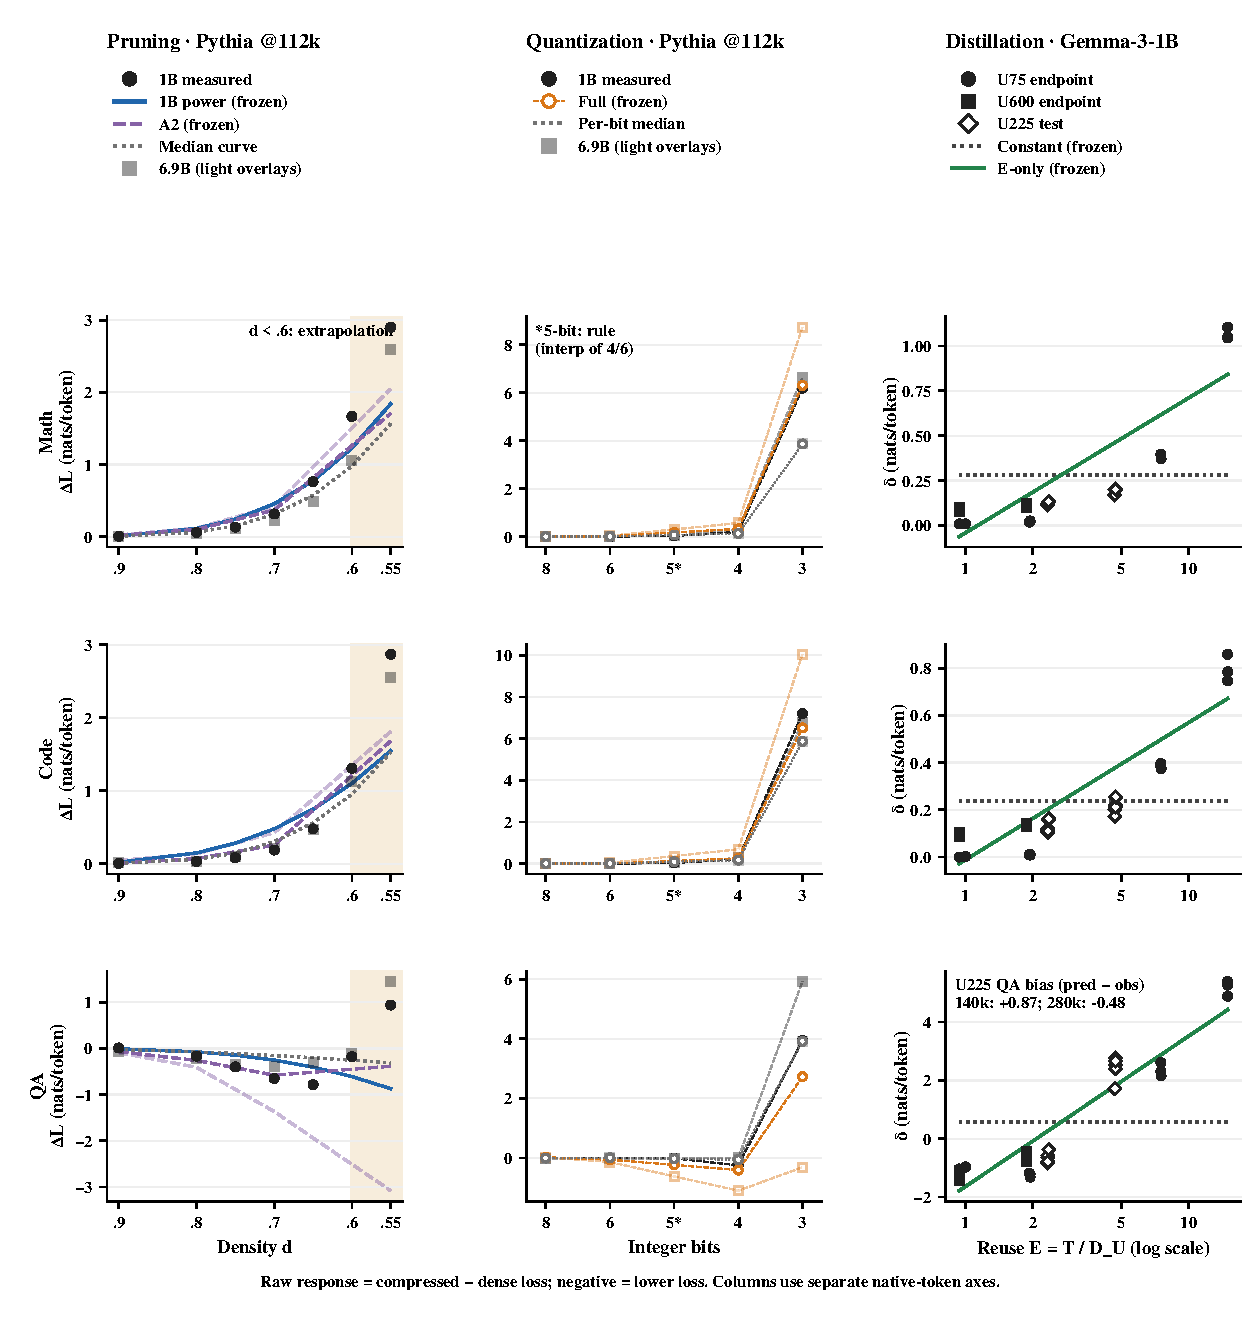
\includegraphics[width=0.88\textwidth]{figs/predictive_responses.pdf}
\caption{Capability-conditioned compression responses and frozen predictions, one source per arm. Left: pruning of Pythia-1B at step 112k (measured, filled circles) with the frozen shared power form (Eq.~\ref{eq:power}), the per-density regression A2, and the source-free median development curve; the 6.9B source at the same stage is overlaid in grey and the extrapolated density $0.55$ is shaded. Middle: per-channel quantization of the same sources at the integer bit-widths with the frozen per-bit regression (hollow) and the per-bit median (dotted); the 5-bit point is the fixed interpolation rule and guide lines are visual only. Right: distillation of Gemma-3-1B, signed transfer $\delta_c$ against the reuse count $E$; endpoint pools U75 and U600 (fit) and the unseen pool U225 (test) with the frozen constant and reuse-count forms and the QA bias at the two budgets. Points are measurements; lines are development fits frozen before the test points were measured. Native nats per token; separate axes per column.}
\label{fig:responses}
\end{figure}

\subsection{Conditioning on the Initial Model State}
\label{sec:conditioning}

The first question is whether the initial state is worth reading at
all, and which part of it carries the signal. On the nine-state
controlled panel, with the intervention setting fixed and one
pretraining stage held out, a regression of the response on
$(N_0,D_0,L_{0,c})$ at each setting lowers the pruning error from
0.413, 0.516, and 0.500 nats (the strongest source-free reference) to
0.253, 0.292, and 0.806 for math, code, and QA; the improvement
interval excludes zero for code, includes zero for math, and is
negative for QA, where predicting no change is better. Input
ablations say which term matters (Fig.~\ref{fig:inputs}A). Adding the
dense capability anchor $L_{0,c}$ to $(N_0,D_0)$ has intervals above
zero for math ($+0.55$, $[0.29,1.00]$) and code ($+0.66$,
$[0.38,1.13]$); adding $D_0$ to $(N_0,L_{0,c})$ does not ($+0.36$,
$[-0.04,0.60]$; $+0.40$, $[-0.01,0.63]$), and for quantization the
$D_0$ increment clears zero in one capability (code) only. A frozen
test at a new stage (step 96k on 160M and 1.4B, between the
development stages) confirmed the same ranking: the full regression
beat both its no-$D_0$ variant and the per-setting median on all three
capabilities. We therefore condition every relation on the three
inputs, read the dense anchor as the carrier of the signal, and keep
$D_0$ as a weak second-order term. The anchor is used per capability;
no joint capability vector is fitted, and nothing here shows that one
would be needed.

\input{tables/models_domains}
\subsection{Pruning}
\label{sec:law_prune}

\paragraph{Response.} Pruning damage grows with the removed fraction
$1-d$ and is source-dependent in amplitude: at the same density a
late-stage small model can be several times more fragile than an
early-stage one, and QA can improve while math and code degrade
(Fig.~\ref{fig:responses}, left). The relation to build is therefore
a source-conditioned amplitude times a strength profile.

\paragraph{Functional form.} The candidate we develop is
\begin{equation}
\widehat{\Delta L}_c(\mathbf x,d)=A_c(\mathbf x)\,\Big(\frac{1-d}{0.3}\Big)^{\gamma_c},
\qquad
A_c(\mathbf x)=\beta_c\cdot\big(1,\tilde{\log N_0},\tilde L_{0,c},\tilde{\log D_0}\big),
\label{eq:power}
\end{equation}
five parameters per capability, where tildes denote standardization on
the development set (Table~\ref{tab:models} summarizes every delivered
predictor). Its same-input alternatives are the per-density
regression A2, which fits $\beta_{c,d}$ separately at each development
density and predicts an unseen $d$ by linear interpolation between the
predicted anchors (four coefficients per density, twenty in total),
the power form with $\gamma_c$ fixed to one, and a continuous two-term
polynomial in $1-d$. The source-free references are a strength-only
curve $A((1-d)/0.3)^{\gamma}$, the median development curve, and zero
change.

\paragraph{Parametric fit and selection.} Fit on the nine development
states at $d\in\{0.9,0.8,0.7,0.6\}$ and evaluated at the pooled unseen
densities $0.65$ and $0.55$, Eq.~\eqref{eq:power} cuts the error of the
strength-only curve by a factor of two to three on every capability, so
reading the source state is what matters, while A2 is better on math
and code and within noise on QA (Table~\ref{tab:pred_main}), so the
power structure adds nothing over the per-density regression. After the
frozen tests of \S\ref{sec:general} we refit both on an expanded
development set of 17 states including the unblinded 1B and 6.9B
checkpoints and applied a pre-committed leave-one-source-out rule: A2
(0.479) and the power form (0.494) tie within 0.02 nats, and the rule
prefers the continuous five-parameter form that vanishes at $d=1$.
Eq.~\eqref{eq:power} with the coefficients of
Appendix~\ref{sec:app_coef} is the delivered pruning predictor; the
exponent $\gamma_c$ is a fitted constant per capability whose
particular value is not established as necessary by these data.

\subsection{Quantization}
\label{sec:law_quant}

\paragraph{Per-bit source regression.} Bit-width alone offers little
room for a continuous relation: int8 and int6 stay within 0.01 nats of
dense, int4 costs 0.03 to 0.35 nats on most states, and int3 collapses
most models by several nats (Fig.~\ref{fig:responses}, middle). The
relation we develop at fixed bit-width is the source regression of
\S\ref{sec:conditioning} applied per bit, four coefficients per
bit-width; it predicts a new state at a seen bit-width and is not a
law over $b$. On the development panel it improves on the per-bit
median for math and code with an interval above zero for code, and
not for QA. The fixed shape $q_c4^{-b}$ misfits this quantizer, whose
integer range uses $q_{\max}=2^{b-1}-1$ levels per sign, and a learned
exponential fits held-out bits better; neither is used as a
predictor.

\paragraph{Group size as a second axis.} A grouped quantizer whose
scale is shared by $g$ contiguous weights changes the error at a fixed
bit-width and is known before the operation, so it adds a genuine
configuration axis. On six development states at $b\in\{3,5\}$ and
$g\in\{64,256\}$ the response has structure: 5-bit cells stay within
0.1 nats, 3-bit damage grows steeply with training stage (late 160M
collapses by 15 to 17 nats, late 1.4B loses 0.6 to 2.2) and roughly
halves when $g$ drops from 256 to 64. Three relations were fit on those
24 cells with the same inputs $\mathbf x$: a separable form
$A_c(\mathbf x)\,q_{\max}^{-p_c}(g/128)^{q_c}$ (six parameters), a
low-order two-dimensional form
\begin{equation}
\widehat{\Delta L}_c(\mathbf x,b,g)=\phi(\mathbf x)\cdot\big[1,\,u,\,v,\,uv,\,u^2\big],
\qquad u=\log_2 q_{\max}(b)\ \text{(centred)},\ v=\log_2\frac{g}{128},
\label{eq:quant2d}
\end{equation}
with one four-vector of state coefficients per term (twenty
parameters), and a same-input bilinear interpolation between the four
development configurations. With only six states the
leave-one-state-out errors are large for all three (the late 160M
collapse dominates them), so the development set does not select a
form; the tests of \S\ref{sec:unseen_settings} do.

\subsection{Distillation}
\label{sec:law_distill}

\paragraph{Response and coordinates.} The response is the signed
transfer $\delta_c$ of an existing student to teacher traces,
relative to the student's own dense loss; the teacher and the size gap
between teacher and student never enter it. Its coordinates are the
supervised completion tokens $T$, the pool size $D_U$ (the completion
tokens of the $U$ traces per domain), and the reuse count $E=T/D_U$;
processed tokens and optimizer steps are recorded separately and never
substituted for $T$. QA improves under every recipe we ran while math
and code respond by a few hundredths to a few tenths of a nat, and
with a small pool the QA loss rises again once $E$ grows large
(Fig.~\ref{fig:responses}, right). The QA improvement is measured on a
multi-hop probe whose format the teacher pool shares; an independent QA
benchmark scored on the same checkpoints did not show it
(Appendix~\ref{sec:app_measure}, Table~\ref{tab:p3_check}), so the
distillation QA response is specific to that probe distribution.

\paragraph{Source axis.} On the nine Pythia states as students, with
the teacher pool and budget fixed, a linear form
$\delta_c=\beta_c\cdot(1,\tilde{\log N_0},\tilde L_{0,c},\tilde{\log D_0})$
halves the error of a per-capability constant for math (0.014
against 0.031 with one stage held out), ties it for code (0.057
against 0.061), and is worse than a constant for QA (0.263 against
0.159). The student state therefore carries the math response and not
the QA response.

\paragraph{Pool and budget axis.} For a fixed student (Gemma-3-1B) we
fit four forms on the endpoint pools U75 and U600: a constant,
$a_c+b_c\log T$, $a_c+b_c\log E$, and $a_c+b_c\log T+c_c\log E$, all
on the positive-budget range of those runs. Their independent test on
an unseen pool is reported in \S\ref{sec:unseen_settings}. With the
complete development matrix of the absolute-exposure protocol (two
students, two pools, three pool samples, four checkpoints) we also
compared two forms that vanish at $T=0$ and carry a student
descriptor $z_c=\tilde L_{0,c}$,
\begin{equation}
\widehat\delta_c=(a_c+\lambda_c z_c)\log(1+E),\qquad
\widehat\delta_c=(a_c+\lambda_c z_c)\big(1-e^{-T/T_*}\big)+(b_c+\mu_c z_c)\log(1+E),
\label{eq:kdforms}
\end{equation}
by leave-one-run-out cross-validation: the first has the lowest math
and code error (0.057 and 0.052 against 0.073 and 0.055 for
$\log(1+E)$ alone), the second the lowest QA error (0.706 against 0.798
for the reuse term alone and 1.40 for a constant). These are
development results on two students; their predictions were specified
after the frozen test matrix and are evaluated on it retrospectively
(Appendix~\ref{sec:app_forms}). No joint student-pool-budget law is
claimed.

\paragraph{Multi-student test.} The joint form with a source term
$k\log(N_S/N_{\mathrm{ref}})$ had the lowest development error of the
eight frozen forms for every capability; on the nine frozen test
trajectories it predicts the unseen pool on both development students
and the held-out 4B student for code and math, and fails for QA on that
student, where the source term extrapolates beyond the two-student
range (Table~\ref{tab:p2v2_test}, \S\ref{sec:unseen_states}). The
delivered distillation law is thus the joint form in $T$ and $E$ with
the source term restricted to the development size range.
